\chapter{Аналитический раздел}
В этом разделе будут рассмотрены определения букмекерской конторы, принципы её функционирования и требования к базе данных, обеспечивающих её работу.

\section{Основные определения}
В статье 4 Федерального Закона от 29.12.2006 N 244-ФЗ (ред. от 02.07.2021) "О государственном регулировании деятельности по организации и проведению азартных игр и о внесении изменений в некоторые законодательные акты Российской Федерации" содержатся следующие определения \cite{bk}:

\textbf{Азартная игра} -- основанное на риске соглашение о выигрыше, заключенное двумя или несколькими участниками такого соглашения между собой либо с организатором азартной игры по правилам, установленным организатором азартной игры \cite{bk}.

\textbf{Пари} -- азартная игра, при которой исход основанного на риске соглашения о выигрыше, заключаемого двумя или несколькими участниками пари между собой либо с организатором данного вида азартной игры, зависит от события, относительно которого неизвестно, наступит оно или нет \cite{bk}.

\textbf{Интерактивная ставка} - денежные средства, в том числе электронные денежные средства, передаваемые с использованием электронных средств платежа, в том числе посредством информационно-телекоммуникационных сетей, включая сеть "Интернет" \cite{bk}.

\textbf{Букмекерская контора} - игорное заведение, в котором организатор азартных игр заключает пари с участниками данного вида азартных игр \cite{bk}.

\section{Принцип работы букмекерской конторы}
Букмекерская контора предлагает игрокам заключить пари на различные события. 
Тип событий может быть различным, но почти всегда букмекерская линия представлена спортивными соревнованиями.
Спорт доминирует на рынке, так как является непредсказуемым, матчи происходят каждый день, и по всему миру живёт огромное количество болельщиков.

Букмекерская контора предлагает коэффициенты на возможные исходы события. Например, в случае футбольного матча такими исходами является победа одной из команд или ничья. Игрок имеет возможность заключить с конторой пари на наступление какого-либо исхода, сделав ставку. Если этот исход наступил, то букмекерская контора должна вернуть игроку денежные средства на сумму, умноженную на коэффициент исхода. В противном случае букмекерская контора оставляет сумму ставки у себя \cite{kfs}.

Рассмотрим первое приближение выбора коэффициента. Пусть $p$ - вероятность наступления какого-либо исхода. Тогда коэффициент рассчитывается по формуле \ref{first}: 
\begin{equation}\label{first}
k = \frac{1}{p}
\end{equation}

Пусть $N$ -- количество ставок игрока, а $S$ -- сумма одной ставки. Математическое ожидание заработка игрока можно посчитать по формуле \ref{win}:
\begin{equation}\label{win} 
M = k_1 * S * p * N - S * N = \frac{1}{p} * S * p * N - S * N = 0
\end{equation}

Так как выигрыш букмекера формируется из проигрыша игрока, из \ref{win} следует, что и математическое ожидание заработка букмекера тоже равняется нулю.

Но букмекерская контора рассчитывает зарабатывать и в краткосрочной, и в долгосрочной перспективе. Для получения прибыли в каждом матче в коэффициенты закладывается маржа. Пусть $p_{win}$ - процент маржи, которые контора хочет иметь, а $\omega$ -- количество исходов события. Тогда коэффициент рассчитывается по формуле \ref{second}:
\begin{equation}\label{second}
k = \frac{1}{p + \frac{p_{win}}{\omega}}
\end{equation}

В таком случае математическое ожидание заработка игрока будет отрицательным, так как коэффициент стал меньше, чем в \ref{first}. Исходя из этого, букмекерская контора остаётся в выигрыша при наступлении любого исхода.

Для того, чтобы постоянно зарабатывать, букмекерам требуется безошибочно рассчитывать вероятности наступления всех событий. 
Этим обычно занимаются профессиональные аналитики и статистики.

Теперь рассмотрим событие, в котором есть два противоположных исхода -- выигрыш одной из команд. Пусть $k_1$ и $k_2$ -- коэффициенты на эти исходы, а $S_1$ и $S_2$ -- денежная сумма, поставленная на эти исходы. 
Если реализуется первый исход, то заработок БК составит $S_1 + S_2 - k_1 * S_1$, а если второй исход -- 
$S_1 + S_2 - k_2 * S_2$. 

Денежные потоки могут быть распределены таким образом, что их распределение не будет соответствовать рассчитанным вероятностям наступления событий. 
В таком случае при наступлении одного из событий БК потеряет деньги.
Следовательно, требуется постоянно обновлять коэффициенты, опираясь на объём средств, поставленных игроками на каждый исход.

При этом всём на букмекерском рынке большая конкуренция, следовательно, требуется предлагать самые выгодные коэффициенты на рынке.

Подводя итог, расчёт коэффициентов на матчи -- сложная математическая, экономическая и маркетинговая задача, которая и позволяет букмекерам зарабатывать деньги \cite{kfs}.

\section{Основные роли в букмекерской конторе}
Букмекерская контора заключает пари с игроками, поэтому первая роль, которая требуется -- \textbf{игрок}. 
Для игроков требуется добавить возможность просмотра линии событий, заключения пари, пополнение баланса, изменения личных данных.
При этом нужно добавить регистрацию, чтобы новый игрок мог воспользоваться аккаунтов, только лишь загрузив приложение. 

Согласно закону № 115-ФЗ «О противодействии легализации (отмыванию) доходов, полученных преступным путем, и финансированию терроризма» об азартных играх, букмекерская контора должна обязательно проводить процедуру идентификации клиентов \cite{bk2}. 
Обычно в букмекерских конторах есть администраторы, которые проверяют указанные игроком данные, и верифицируют аккаунтов. 
Лишь после этого у клиента есть возможность совершать ставки на какие-либо события.
Поэтому следующая роль -- \textbf{администратор}.

В его функционал входит верификация новых пользователей или отклонение заявки игрока.
Подразумевается, что администратор имеет доступ к какой-то сторонней базе данных, где может проверить паспортные данные, однако это выходит за пределы курсовой работы.
Поэтому администратор просто имеет возможность изменить статус игрока.

Также в букмекерской конторе кто-то должен заниматься линией матчей. 
Требуется добавлять новые матчи в линию, изменять их статус (событие началось, закончилось), менять текущий счёт и изменять коэффициенты.
Этим занимается \textbf{аналитик}, который имеет возможность добавлять события в линию и менять о них информацию.

Use-Case диаграмма ролей проекта представлена на рисунке \ref{fig::UseCase}:

\FloatBarrier
\begin{figure}[hp]	
	\begin{center}
		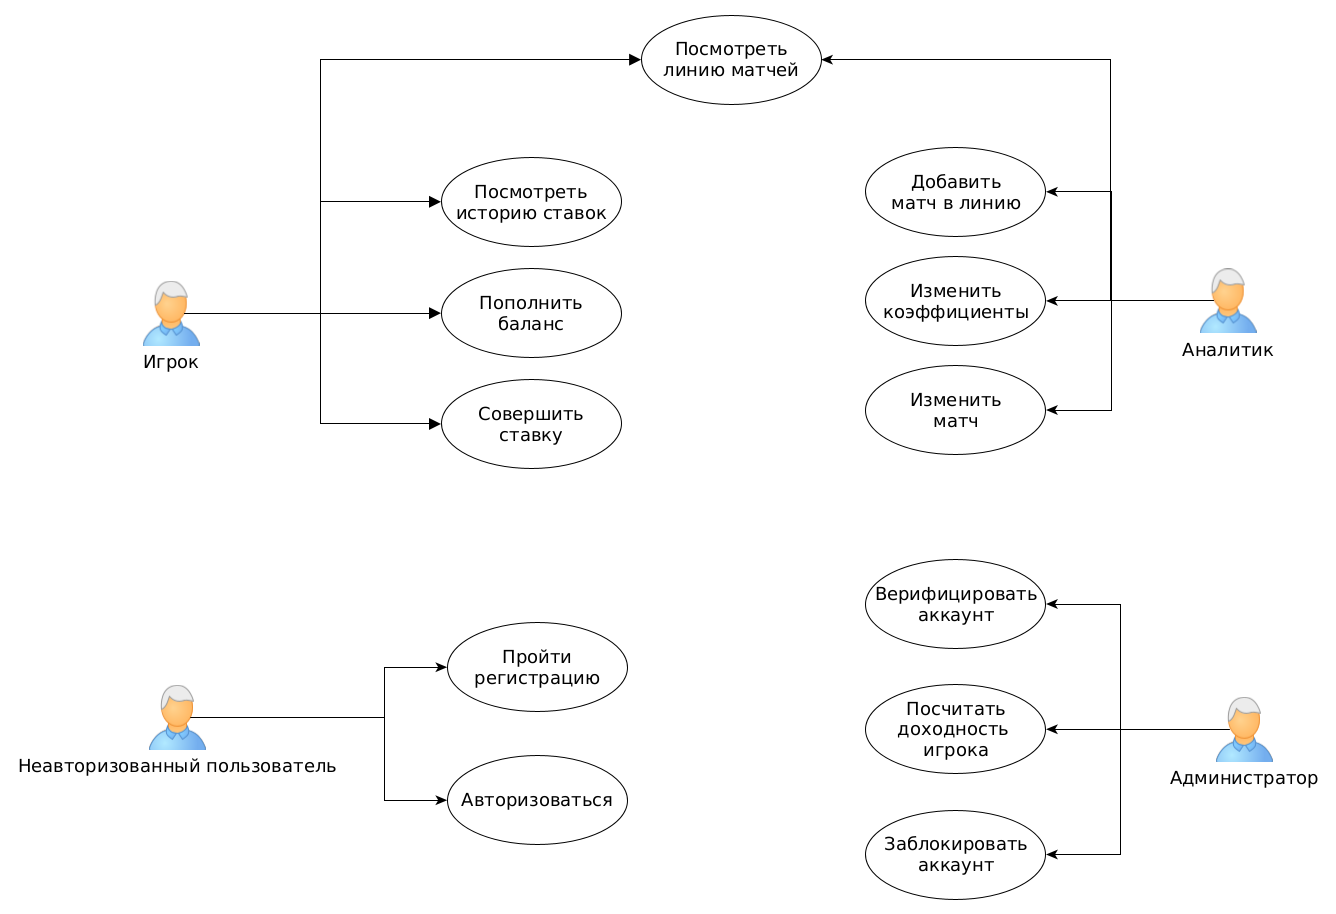
\includegraphics[width=\linewidth]{inc/useCase.png}
	\end{center}
	\caption{Use-Case диаграмма}
	\label{fig::UseCase}
\end{figure}
\FloatBarrier


\section{Цикл одного события в букмекерской конторе}
Для обеспечения работы букмекерской платформы требуется, чтобы игроку был предоставлен выбор из событий.
Требуется, чтобы аналитик добавил событие в букмекерской конторе. 
Событие происходит в абстрактном виде спорта, в котором возможно три исхода: победа первой команды, ничья, и победа второй команды. 
У каждого события есть дата и время начала, две команды, которые встречаются в матче, а также коэффициенты на каждый из исходов.
Аналитик должен указать все данные события. 
Для упрощения работы, список команд должен быть постоянным, и храниться в базе данных. 
При этом в одном событии не может быть двух одинаковых команд, а коэффициенты на исход должны соответствовать теоретическим изложениям из п.1.2 настоящего РПЗ.

У каждого события есть атрибут статуса. Всего есть три варианта:
\begin{enumerate}
	\item Событие запланировано, но ещё не началось.
	\item Событие идёт в текущий момент.
	\item Событие закончилось.
\end{enumerate} 

Аналитику требуется своевременно вносить правки в статус матча: изменять статус события, изменять счёт встречи, а также менять коэффициенты в зависимости от того, как складывается встреча.

Как только аналитик пометил событие законченным, у матча меняется статут на "закончен", и букмекерская контора должна рассчитать тех, кто выиграл пари, и заплатить им.

\section{Требования к базе данных букмекерской конторы}
Платформа для обеспечения работы букмекерской конторы должна использовать базу данных для нескольких целей:
\begin{enumerate}
	\item Хранения информации о пользователях, их балансе и личной информации.
	\item Хранения информации о событиях в линии, причём как запланированных и текущих, так и о законченных.
	\item Хранения информации о совершённых игроком ставок для прозрачности работы конторы.
	\item Автоматического обновления баланса игроков при заключении пари и перерасчёта в случае выигрыша.
	\item Хранения информации об аккаунтах и ролях, связанных с ними.
	\item Различий в возможностях ролей при работе с базой данных.
\end{enumerate}

Также требуется обратить внимание на следующие детали при разработке базы данных:
\begin{itemize}
	\item данные в букмекерской конторе не должны быть избыточны, следовательно, требуется привести отношения к нормальной форме;
	\item букмекерская контора хранит персональные данные пользователей, следовательно, требуется обеспечить безопасность работы с паспортными данными, паролями, чтобы их было невозможно получить нежелательным лицам;
	\item так как состояние матча также хранится в БД, автоматическое обновление баланса игроков можно реализовать при помощи триггеров на определённые события;
	\item ставка может считаться сделанной, если информация о ней записана в БД и с баланса игрока списаны средства, равные размеру ставки. При этом коэффициент может измениться во время работы системы. Поэтому требуется использовать транзакции для поддержки функционала заключения пари.
\end{itemize}

\section{Основные отношения в базе данных}
В соответствии с вышеперечисленными аспектами базы данных для платформы, в БД должны быть представлены следующие отношения с атрибутами:
\begin{enumerate}
	\item \textbf{Аккаунты}. В качестве информации должен храниться логин и пароль для входа в систему, а также роль, соответствующая аккаунту. Это отношение может быть изменено напрямую только администратором. Также оно автоматически обновляется при регистрации нового игрока.
	\item \textbf{Пользователи}. В этом отношении должна храниться основная личная информация о пользователе: номер телефона, электронная почта, номер паспорта. Также оно содержит информацию о балансе игрока и максимальной ставке. Предполагается, что букмекерская контора будет иметь возможность порезать счёт успешного игрока, существенно уменьшив собственные убытки.
	\item \textbf{Команды}. В этом отношении должны храниться команды, которые могут быть в событии. В качестве атрибутов рассматривается название, логотип и город.
	\item \textbf{События}. В этом отношении хранятся все события: дата создания, их статус, итоговый счёт, команды, принимающие участия. 
	\item \textbf{Ставки}. В этом отношении хранятся все совершённые ставки и события.
\end{enumerate}

Концептуально отношения в базе данных можно представить с помощью ER-модели нотации Чена.
На рисунке \ref{fig::chen} представлена ER-модель в нотации Чена:
\FloatBarrier
\begin{figure}[hp]	
	\begin{center}
		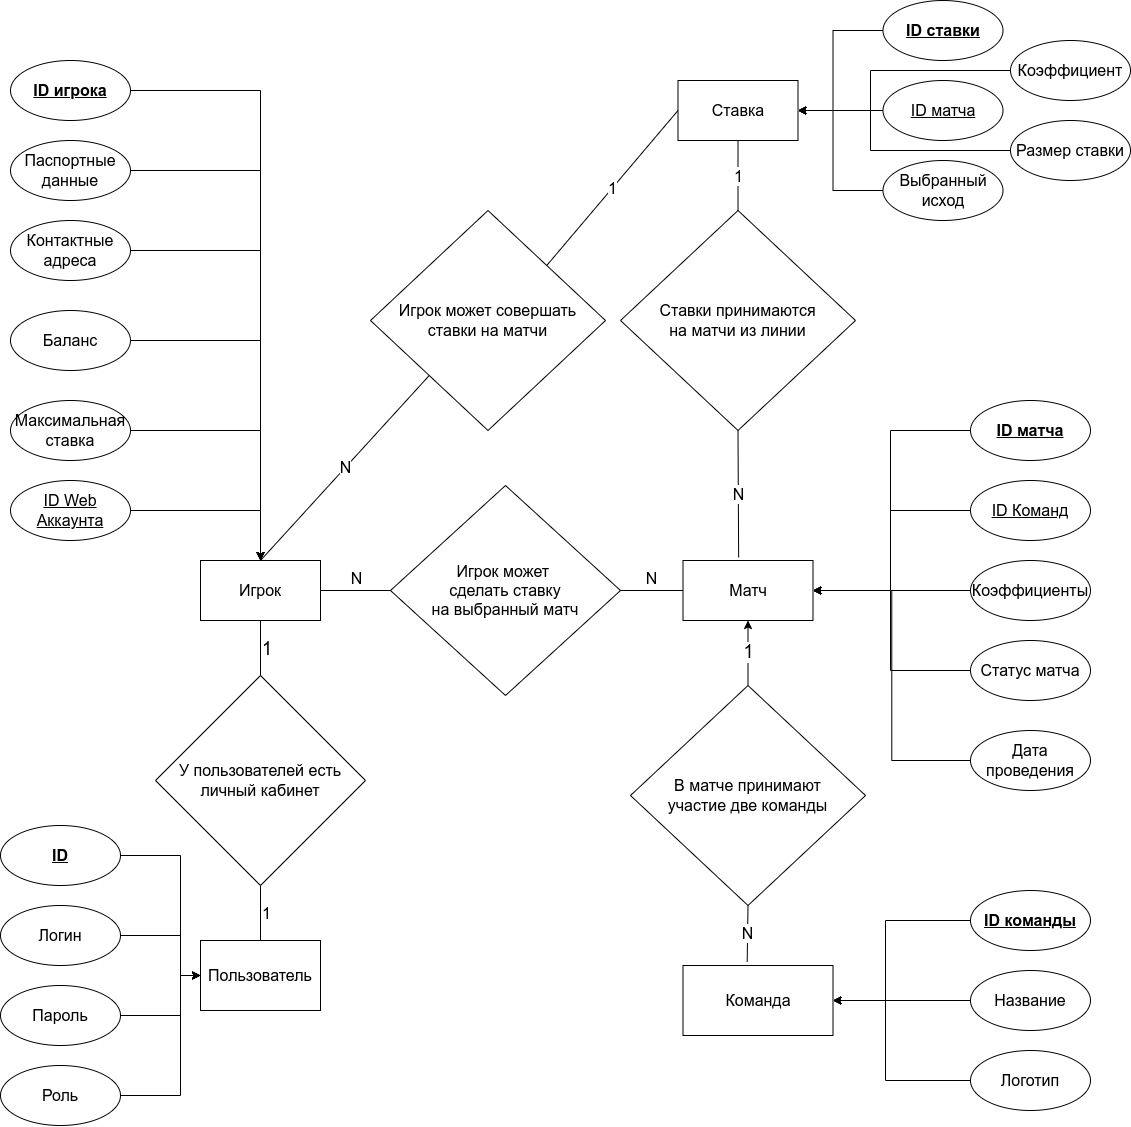
\includegraphics[width=\linewidth]{inc/chen.png}
	\end{center}
	\caption{ER-модель в нотации Чена}
	\label{fig::chen}
\end{figure}
\FloatBarrier
